%==============================================================================
% Sjabloon onderzoeksvoorstel bachelorproef
%==============================================================================%
% Compileren in TeXstudio:
%
% - Zorg dat Biber de bibliografie compileert (en niet Biblatex)
%   Options > Configure > Build > Default Bibliography Tool: "txs:///biber"
% - F5 om te compileren en het resultaat te bekijken.
% - Als de bibliografie niet zichtbaar is, probeer dan F5 - F8 - F5
%   Met F8 compileer je de bibliografie apart.
%
% Als je JabRef gebruikt voor het bijhouden van de bibliografie, zorg dan
% dat je in ``biblatex''-modus opslaat: File > Switch to BibLaTeX mode.

\documentclass{hogent-article}
\usepackage{graphicx}
\usepackage{lipsum} % Voor vultekst


%------------------------------------------------------------------------------
% Metadata over het artikel
%------------------------------------------------------------------------------

%---------- Titel & auteur ----------------------------------------------------

% TODO: (fase 2) geef werktitel van je eigen voorstel op
\PaperTitle{Machine learning applicatie voor de detectie  van slaapbruxisme}
% Dit is typisch de opdracht en het vak waarvoor dit artikel geschreven is, bv.
% ``Verslag onderzoeksproject Onderzoekstechnieken 2018-2019''
\PaperType{Paper Research Methods: onderzoeksvoorstel}

% TODO: (fase 1) vul je eigen naam in als auteur, geef ook je emailadres mee!
\Authors{Brent De Corte\textsuperscript{1}} % Authors

% Als het hier effectief gaat om een voorstel voor de bachelorproef, dan ben je
% hier verplicht de naam van je co-promotor in te vullen. Zoniet, dan kan je het
% leeg laten.
\CoPromotor{}

% Contactinfo: Geef hier de contactgegevens van elke auteur van het artikel (en
% indien van toepassing ook van de co-promotor).
\affiliation{
  \textsuperscript{1} \href{mailto:brent.decorte@student.hogent.be}{brent.decorte@student.hogent.be}}


%---------- Abstract ----------------------------------------------------------

\Abstract{% TODO: (fase 6)
Dit onderzoek zal zich focussen op de creatie van een audiodetectiesysteem via een deep learning model dat zal worden geïntegreerd in een mobiele applicatie, met als doelstelling het vaststellen van Bruxisme door het onderscheiden en vastleggen van het typisch knarsend geluid van tanden.
Het model komt tot stand door de transformatie van audiofragmenten in spectrogrammen met extra tijd en maakt gebruik van een filter op basis van geluidsfrequenties waardoor het scenario in een beeldclassificatie kan omgezet worden . Van zodra het model ontwikkeld is, zal het worden geïmplementeerd in een mobiele applicatie welke gebaseerd is op het Python framework Kivy .}

%---------- Onderzoeksdomein en sleutelwoorden --------------------------------
% TODO: (fase 2) Vul de sleutelwoorden aan.

% Het eerste sleutelwoord beschrijft het onderzoeksdomein. Je kan kiezen uit
% deze lijst:
%
% - Mobiele applicatieontwikkeling
% - Webapplicatieontwikkeling
% - Applicatieontwikkeling (andere)
% - Systeembeheer
% - Netwerkbeheer
% - Mainframe
% - E-business
% - Databanken en big data
% - Machineleertechnieken en kunstmatige intelligentie
% - Andere (specifieer)
%
% De andere sleutelwoorden zijn vrij te kiezen.

\Keywords{Machineleertechnieken en kunstmatige intelligentie; geluiddetectie; Bruxisme}
\newcommand{\keywordname}{Sleutelwoorden} % Defines the keywords heading name

%---------- Titel, inhoud -----------------------------------------------------

\bibliography{bibliografie}

\begin{document}



\flushbottom % Makes all text pages the same height
\maketitle % Print the title and abstract box
\tableofcontents % Print the contents section
\thispagestyle{empty} % Removes page numbering from the first page

%------------------------------------------------------------------------------
% Hoofdtekst
%------------------------------------------------------------------------------

\section{Inleiding}

% TODO: (fase 2) introduceer je gekozen onderwerp, formuleer de onderzoeksvraag en deelvragen. Wat is de doelstelling (is die S.M.A.R.T.?), wat zal het resultaat zijn van het onderzoek (een Proof-of-Concept, een prototype, een advies, ...)? Waarom is het nuttig om dit onderwerp te onderzoeken?
Slaapbruxisme (SB) is het onbewust over elkaar heen en weer  schuiven van de boven- en onderkaak, zodat de tanden een schurend en knarsend geluid voortbrengen. SB kan leiden tot heel wat complicaties waaronder hypertensie, disfunctie van het kaak- en tandstelsel, gebitsproblemen met o.a. het verlies van tandoppervlakte en gebarsten tanden, het slecht slapen en hoofdpijn. Deze gevolgen kunnen leiden tot een noemenswaardige daling van de levenskwaliteit.  Daarom is het essentieel om snel en gemakkelijk vast te kunnen stellen of  iemand  aan  SB lijdt .
\bigbreak
\noindent
Er zijn enkele apparaten verkrijgbaar op de markt die  de mogelijkheid bieden om thuis SB vast te stellen, dit op basis van kaak- en spiermetingen of zenuwmetingen. Een voorbeeld hiervan is de BiteStrip \cite{Shochat_2007}.  Deze methode van detectie is adequaat, maar heeft tekortkomingen zoals de kost van de apparatuur en het limiteren van de slaap tijdens het detectieproces . 
\bigbreak
\noindent
Omdat er tot op heden nog geen eenvoudig detectiesysteem bestaat dat prijsvriendelijk en betrouwbaar is en  dat het slaapproces niet hindert, zou het toepassen van Machine learning een gewenste oplossing bieden voor het tijdig vaststellen van SB.








\section{Overzicht literatuur}

% TODO: (fase 4) schrijf de literatuurstudie uit en gebruik waar gepast referenties naar de vakliteratuur.

% Refereren naar de literatuur kan met:
% \autocite{BIBTEXKEY} -> (Auteur, jaartal)
% \textcite{BIBTEXKEY} -> Auteur (jaartal)
%Voorbeeld van een referentie waar de auteursnaam geen onderdeel van de zin is~\autocite{Moore2002}.
Vandaag bestaan er verschillende methodes om SB te ontdekken zoals deze op basis van een electromyografie, waarbij elektrische signalen van de zenuwen worden omgezet in interpreteerbare data en het registreren van een toegenomen hartslag voordat een SB-aanval begint.  Dit staat omschreven in  \cite{Deregibus_2013}.  Ook bestaat er een methode die zich baseert op het meten van kaak- en spierbewegingen zoals vermeld in \cite{Shochat_2007}  .  Beide van deze methodes zijn gelimiteerd in hun manier van detecteren, omdat ze het slaapcomfort van de patiënt verminderen. \bigbreak
\noindent
Om de hoeveelheid opgenomen data te verhogen, zijn  er verschillende methodes, o.a. :



\begin{itemize}

	
	\item Time stretching \autocite{Wei_2020}
	\bigbreak 
	\begin{itemize}
		\item Het verhogen of verlagen van de snelheid waarmee het audiofragment wordt afgespeeld. Om de originele inputgrootte van het model te behouden kan zero-padding worden gebruikt als het fragment versneld wordt of cropping als het fragment vertraagd wordt.
		 
	\end{itemize}
	\bigbreak
	\item toevoegen van "noise" \autocite{Wei_2020}
	\bigbreak
	\begin{itemize}
		\item De toevoeging van Gauss-ruis met de hyperparameter die de amplitude regelt, laat de mogelijkheid om overfitting tegen te gaan. \newline Het gebruik van Gauss-ruis is niet gelimiteerd tot de input maar kan ook toegevoegd worden aan de andere componenten zoals de activatiefunctie.
	\end{itemize}
	\bigbreak
	\break
	\item pitch shift \autocite{Wei_2020}
	\bigbreak 
	\begin{itemize}
		\item Het verhogen of verlagen van de halve toonafstanden, de kleinste stap omhoog of omlaag van een bestaande toon van het audiofragment.  Dit is hetzelfde concept als het hierboven vermelde Time Stretching.
			
	\end{itemize}
	\bigbreak

	\item SpecAugment \autocite{Park_2019}
	\bigbreak
	\begin{itemize}
		\item SpecAugment gebruikt 2 methodes om spectro- grammen uit te breiden.  Het verbergen van een bepaald bereik op de frequentieschaal, frequency masking genoemd en het verbergen van een bereik op de tijdschaal, time masking genoemd.
		Deze 2 methodes maken samen het uiteindelijke model  resistenter tegen het verlies van informatie. 
		
		
		
	\end{itemize}
\end{itemize}
\bigbreak
\noindent
Nog andere audiodetectiesystemen bestaan waaronder een  hoestdetector, omschreven in \cite{Kvapilova_2019}.  Hier wordt de  data opgesplitst in fragmenten van 1 seconde. Deze fragmenten worden omgezet in spectrogrammen door het gebruik van de Fourier-methode. Deze spectrogrammen  dienen om een convolutioneel netwerk te trainen.

.


\section{Methodologie}

% TODO: (fase 5) beschrijf in detail in welke fasen je onderzoek uiteenvalt, hoe lang elke fase duurt en wat het concrete resultaat van elke fase is. Welke onderzoekstechniek ga je toepassen om elk van je onderzoeksvragen te beantwoorden? Gebruik je hiervoor experimenten, vragenlijsten, simulaties? Je beschrijft ook al welke tools je denkt hiervoor te gebruiken of te ontwikkelen.
\subsection{Observatie}

In het stadium van observatie zijn de noodzakelijke vereisten het verzamelen, verwerken en het labelen van de data. Het verzamelen van de data gebeurt tijdens verschillende sessies, door het opnemen van  klanken van personen met en zonder SB tijdens hun slaapproces.  Ook andere fragmenten zoals het kauwen worden opgenomen. Deze geluiden registreert men via smartphone om zo goed mogelijk de eigenlijke use case te vertegenwoordigen.



\begin{figure}[h!]
    \centering
    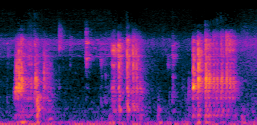
\includegraphics[width=0.7\linewidth]{brux_spec}
    \caption{ spectrogram van tandenknarsen (duratie 3s mono)}
    \label{fig:mil spectrogram of teeth grinding (duration 3s)}
\end{figure}
\noindent
De verzamelde data kan worden opgesplitst in kleinere fragmenten.
Het aantal fragmenten kan vergroot worden met time stretching en pitch shifting, waarbij rekening moet worden gehouden met de inputgrootte van het model. Het gebruik van Gauss-ruis kan ook worden gebruikt voor augmentatie van de bestaande fragmenten.




\bigbreak
\noindent
Wanneer de data is aangepast en verzameld kan ze worden omgezet in spectrogrammen door het gebruik van time- en frequency masking. Deze methodes zorgen voor een tweeledig voordeel.  Het model is resistenter tegen ontbrekende data omdat het zich moet focussen op de meest essentiële features en heeft daarbij ook het voordeel van de extra uitbreiding van de hoeveelheid spectrogrammen. Wanneer de spectrogrammen  aangemaakt zijn worden ze gelabeld. De spectrogrammen geven de mogelijkheid om het als een image-classificatieprobleem op te lossen.

\bigbreak
\noindent
Alle data zal worden opgeslagen gebruik makend van MongoDb in de aangepaste vorm om de waarborg van privacy van de subjecten te garanderen.
\bigbreak
\noindent
Nadat de data werd verwerkt en bewaard kan een werkend model worden opgebouwd, waar factoren zoals precisie en herinnering belangrijke componenten zijn om het juiste model te selecteren . Het werkend model zal worden geïmplementeerd in een mobiele applicatie als proof of concept . De grootste hoeveelheid van de beschikbare tijd zal worden gespendeerd aan data collectie en verwerking.


\subsection{Proof of concept}

Het PoC zal opgebouwd worden en gebruik maken van het Python framework Kivy. Deze applicatie zal de mogelijkheid bieden om geluid op te nemen en de user op de hoogte brengen hoeveel SB- gebeurtenissen plaatsvonden de afgelopen nacht.


\bigbreak
\noindent
Als samenvatting :  data wordt verzameld van SB- en niet SB-subjecten met een aantal soorten kauwgerelateerde geluiden. Die data wordt verwerkt en omgevormd tot spectrogrammen.  De spectrogrammen laten toe om een image- classificatiesysteem te maken. Het model wordt geïmplementeerd in een mobiele applicatie dat gebruik maakt van Kivy.






\section{Verwachte conclusies}

% TODO: (fase 6) beschrijf wat je verwacht uit je onderzoek en waarom (bv. volgens je literatuuronderzoek is softwarepakket A het meest gebruikte en denk je dat het voor deze casus ook het meest geschikt zal zijn). Natuurlijk kan je niet in de toekomst kijken en mag je geen alternatieve mogelijkheden uitsluiten. In de praktijk gebeurt het ook vaak dat een onderzoek tot verrassende resultaten leidt, dat maakt het proces nog interessanter!

Het ontstaan van een gebruiksvriendelijk en voor iedereen toegankelijke applicatie met een convolutioneel model dat SB-gebeurtenissen detecteert en de duur/ernst ervan opmeet. Met deze App kan vroegtijdig actie ondernomen worden om schade aan de gezondheid te voorkomen.
\noindent
De PoC mobiele applicatie zal gebouwd worden met het Python framework Kivy. 











%------------------------------------------------------------------------------
% Referentielijst
%------------------------------------------------------------------------------
% TODO: (fase 4) de gerefereerde werken moeten in BibTeX-bestand
% bibliografie.bib voorkomen. Gebruik JabRef om je bibliografie bij te
% houden.

\phantomsection
\printbibliography
\noindent\makebox[\linewidth]{\rule{\paperwidth / 3}{0.4pt}}
https://github.com/Brent-dc/Researchmethods
\end{document}
